\apendice{Demonstração do Circuito}
\label{ap:apendiceA}

Com a finalidade de entender o que acontece em cada parte do circuito + será feita a demonstração passo a passo das operações a cada camada.

Seja $\ket{\psi}$ o estado inicial do espaço formado pelos $4$ qubits + com valor inicial dado por $\ket{\psi} = \ket{0000}$. Aplicaremos portas \textit{Hadamard} em cada qubit como parte da primeira etapa do Algoritmo de Grover: a preparação inicial. Essa operação resulta em:

\begin{enumerate}[nosep,leftmargin=*]
    \item Preparação inicial: aplicação das portas \textit{H}'s (Figura~\ref{fig:psi1}):
    \begin{flalign*}
        H^{\otimes 4}\ket{\psi} &= \ket{\psi_1} = \frac{1}{4} \Bigl(\ket{0000} + \ket{0001} + \ket{0010} + \ket{0011} + \ket{0100} + \ket{0101} + \ket{0110} && \\ &
        + \ket{0111} +  \ket{1000} + \ket{1001} + \ket{1010} + \ket{1011} + \ket{1100} + \ket{1101} + \ket{1110} + \ket{1111}\Bigr) &&
    \end{flalign*}
    \vspace{-30pt}
    \begin{figure}[ht!]
        \centering
        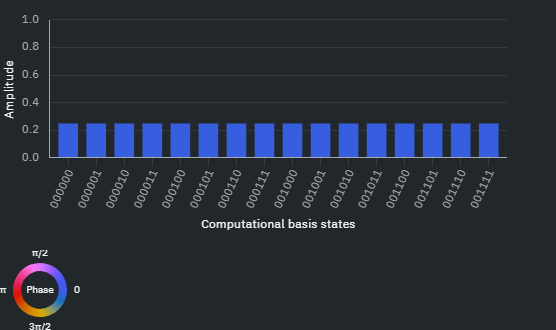
\includegraphics[trim=0mm 47mm 15mm 0mm, clip, width=.6\linewidth]{Imagens/EvPsi/Psi1.png}
        \caption{Aplicação das portas \textit{H}'s na preparação inicial.}
        \label{fig:psi1}
    
    {\small Fonte: IBM-\textit{Quantum Learning / Composer}.}
    \end{figure}
    \item Aplicar o oráculo \(U_f\) que marca o estado \(\ket{1111}\) invertendo seu sinal (Figura~\ref{fig:psi2}):
        \begin{flalign*}
        U_f\ket{\psi_1} &= \ket{\psi_2} = \frac{1}{4} \Bigl(\ket{0000} + \ket{0001} + \ket{0010} + \ket{0011} + \ket{0100} + \ket{0101} + \ket{0110} && \\ & 
        + \ket{0111} + \ket{1000} + \ket{1001} + \ket{1010} + \ket{1011} + \ket{1100} + \ket{1101} + \ket{1110} - \ket{1111}\Bigr) &&
    \end{flalign*}
    \vspace{-30pt}
    \begin{figure}[ht!]
        \centering
        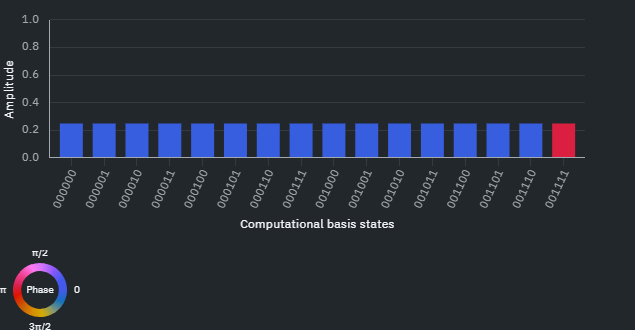
\includegraphics[trim=0mm 47mm 15mm 0mm, clip, width=.6\linewidth]{Imagens/EvPsi/Psi2.png}
        \caption{Aplicação do oráculo \(U_f\), que inverte o sinal do estado \(\ket{1111}\).}
        \label{fig:psi2}
    
    {\small Fonte: IBM-\textit{Quantum Learning / Composer}.}
    \end{figure}

    \item Início da operação de difusão: aplicar portas \textit{Hadamard} (Figura~\ref{fig:psi3}):
        \begin{flalign*}
        H^{\otimes 4}\ket{\psi_2} &= \ket{\psi_3} = \frac{1}{8} \Bigl( 7\ket{0000} + \ket{0001} + \ket{0010} - \ket{0011} + \ket{0100} - \ket{0101} - \ket{0110} && \\ & 
        + \ket{0111} + \ket{1000} - \ket{1001} - \ket{1010} + \ket{1011} - \ket{1100} + \ket{1101} + \ket{1110} - \ket{1111} \Bigr) &&
    \end{flalign*}
    \vspace{-30pt}
    \begin{figure}[ht!]
        \centering
        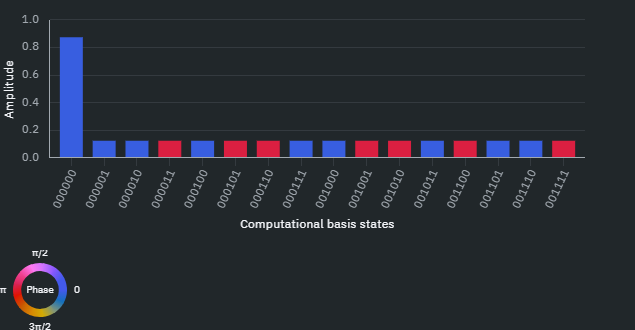
\includegraphics[trim=0mm 47mm 15mm 0mm, clip, width=.6\linewidth]{Imagens/EvPsi/Psi3.png}
        \caption{Aplicação das portas \textit{Hadamard} no início da operação de difusão.}
        \label{fig:psi3}
    
    {\small Fonte: IBM-\textit{Quantum Learning / Composer}.}
    \end{figure}

    \item Aplicar portas $X$ (Figura~\ref{fig:psi4}):
  \begin{flalign*}
        X^{\otimes 4}\ket{\psi_3} &= \ket{\psi_4} = \frac{1}{8} \Bigl( 7\ket{1111} + \ket{1110} + \ket{1101} - \ket{1100} + \ket{1011} - \ket{1010} - \ket{1001} + \ket{1000} && \\ &
        + \ket{0111} - \ket{0110} - \ket{0101} + \ket{0100} - \ket{0011} + \ket{0010} + \ket{0001} - \ket{0000}\Bigr) && \\[6pt]
        &= \frac{1}{8} \Bigl(-\ket{0000} + \ket{0001} + \ket{0010} - \ket{0011} + \ket{0100} - \ket{0101} - \ket{0110} + \ket{0111} && \\ &
        + \ket{1000} - \ket{1001} - \ket{1010} + \ket{1011} - \ket{1100} + \ket{1101} + \ket{1110} + 7\ket{1111}\Bigr) &&
    \end{flalign*}
    \vspace{-30pt}
    \begin{figure}[ht!]
        \centering
        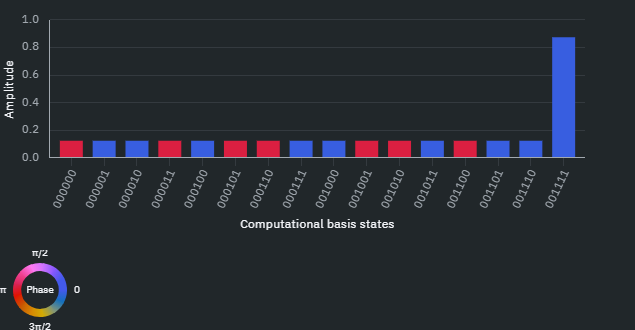
\includegraphics[trim=0mm 47mm 15mm 0mm, clip, width=.6\linewidth]{Imagens/EvPsi/Psi4.png}
        \caption{Aplicação das portas $X$ no operador de difusão.}
        \label{fig:psi4}
    
    {\small Fonte: IBM-\textit{Quantum Learning / Composer}.}
    \end{figure}

    \item Aplicar a porta $MCZ$ (Figura~\ref{fig:psi5}):
        \begin{flalign*}
        MCZ \ket{\psi_4} &= \ket{\psi_5} = \frac{1}{8} \Bigl(-\ket{0000} + \ket{0001} + \ket{0010} - \ket{0011} + \ket{0100} - \ket{0101} - \ket{0110} && \\ 
        + \ket{0111} & + \ket{1000} - \ket{1001} - \ket{1010} + \ket{1011} - \ket{1100} + \ket{1101} + \ket{1110} - 7 \ket{1111}\Bigr) &&
    \end{flalign*}
    \vspace{-30pt}
    \begin{figure}[ht!]
        \centering
        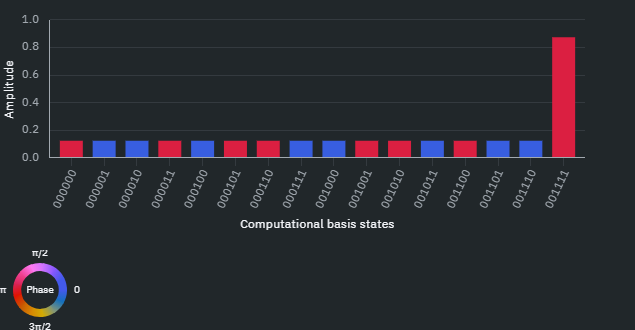
\includegraphics[trim=0mm 47mm 15mm 0mm, clip, width=.6\linewidth]{Imagens/EvPsi/Psi5.png}
        \caption{Aplicação da porta $MCZ$ no operador de difusão.}
        \label{fig:psi5}
    
    {\small Fonte: IBM-\textit{Quantum Learning / Composer}.}
    \end{figure}
    \item Aplicar portas $X$ novamente (Figura~\ref{fig:psi6}):
   \begin{flalign*}
        X^{\otimes 4} \ket{\psi_5} &= \ket{\psi_6} = \frac{1}{8} \Bigl( -\ket{1111} + \ket{1110} + \ket{1101} - \ket{1100} + \ket{1011} - \ket{1010} - \ket{1001}  && \\
        + \ket{1000} & + \ket{0111} - \ket{0110} - \ket{0101} + \ket{0100} - \ket{0011} + \ket{0010} + \ket{0001} - 7 \ket{0000}\Bigr) && \\[6pt]
        &= \frac{1}{8} \Bigl(-7 \ket{0000} + \ket{0001} + \ket{0010} - \ket{0011} + \ket{0100} - \ket{0101} - \ket{0110} + \ket{0111} && \\ & 
        + \ket{1000} - \ket{1001} - \ket{1010} + \ket{1011} - \ket{1100} + \ket{1101} + \ket{1110} - \ket{1111} \Bigr) &&
    \end{flalign*}
    \vspace{-30pt}
    \begin{figure}[ht!]
        \centering
        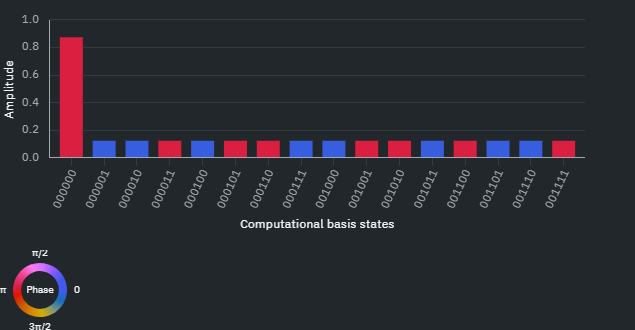
\includegraphics[trim=0mm 47mm 15mm 0mm, clip, width=.6\linewidth]{Imagens/EvPsi/Psi6.png}
        \caption{Segunda aplicação das portas $X$ no operador de difusão.}
        \label{fig:psi6}
    
    {\small Fonte: IBM-\textit{Quantum Learning / Composer}.}
    \end{figure}

    \item Aplicar portas \textit{Hadamard} novamente (Figura~\ref{fig:psi7}):
\begin{flalign*}
    H^{\otimes 4} \ket{\psi_6} &= \ket{\psi_7} = \frac{1}{16} \Bigl( 
        -3\ket{0000} - 3\ket{0001} - 3\ket{0010} - 3\ket{0011} - 3\ket{0100} - 3\ket{0101} && \\ &\quad - 3\ket{0110} - 3\ket{0111} - 3\ket{1000} - 3\ket{1001} - 3\ket{1010} && \\
        & - 3\ket{1011} - 3\ket{1100} - 3\ket{1101} - 3\ket{1110} - 11\ket{1111} 
    \Bigr) && \\[6pt]
    &= -\frac{3}{16} \Bigl(
        \ket{0000} + \ket{0001} + \ket{0010} + \ket{0011} + \ket{0100} + \ket{0101} + \ket{0110} + \ket{0111} && \\
        & + \ket{1000} + \ket{1001} + \ket{1010} + \ket{1011} + \ket{1100} + \ket{1101} + \ket{1110} + \frac{11}{3} \ket{1111}
    \Bigr) &&
\end{flalign*}
    \vspace{-30pt}
    \begin{figure}[ht!]
        \centering
        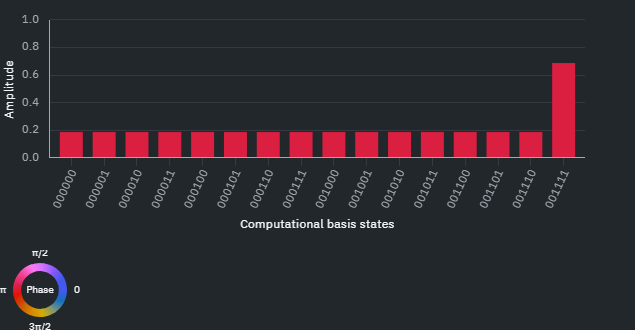
\includegraphics[trim=0mm 47mm 15mm 0mm, clip, width=.6\linewidth]{Imagens/EvPsi/Psi7.png}
        \caption{Aplicação final das portas \textit{Hadamard} na primeira iteração.}
        \label{fig:psi7}
    
    {\small Fonte: IBM-\textit{Quantum Learning / Composer}.}
    \end{figure}

    O sétimo passo finaliza a primeira iteração, mas precisamos repetir o processo mais duas vezes.

    \item Marcar novamente o estado buscado pelo oráculo \(U_f\) (Figura~\ref{fig:psi8}):
    \begin{flalign*}
        U_f \ket{\psi_7} &= \ket{\psi_8} = -\frac{3}{16} \Bigl( \ket{0000} + \ket{0001} + \ket{0010} + \ket{0011} + \ket{0100} + \ket{0101} + \ket{0110} && \\  
         + \ket{0111} &+ \ket{1000} + \ket{1001} + \ket{1010} + \ket{1011} + \ket{1100} + \ket{1101} + \ket{1110} - \frac{11}{3} \ket{1111} \Bigr)
    \end{flalign*}
    \vspace{-30pt}
    \begin{figure}[ht!]
        \centering
        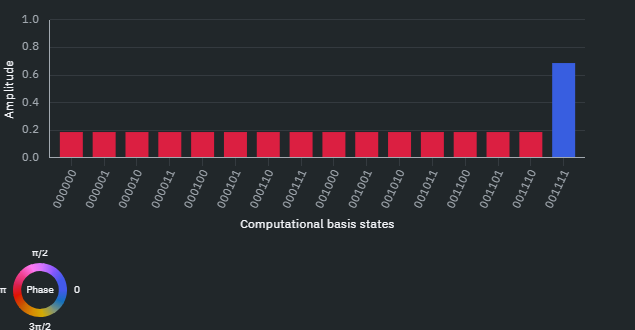
\includegraphics[trim=0mm 47mm 15mm 0mm, clip, width=.6\linewidth]{Imagens/EvPsi/Psi8.png}
        \caption{Aplicação do oráculo \(U_f\) na segunda iteração.}
        \label{fig:psi8}
    
    {\small Fonte: IBM-\textit{Quantum Learning / Composer}.}
    \end{figure}

    Após o oráculo, devemos aplicar o operador de difusão.

    \item Aplicar portas \textit{Hadamard} (Figura~\ref{fig:psi9}):
    \begin{flalign*}
        H^{\otimes 4} \ket{\psi_8} &= \ket{\psi_9} = \frac{7}{32} \Bigl(-\frac{17}{7} \ket{0000} - \ket{0001} - \ket{0010} + \ket{0011} - \ket{0100} + \ket{0101} + \ket{0110} && \\\ &
        - \ket{0111} - \ket{1000} + \ket{1001} + \ket{1010} - \ket{1011} + \ket{1100} - \ket{1101} - \ket{1110} + \ket{1111} \Bigr)
    \end{flalign*}
    \vspace{-30pt}
    \begin{figure}[ht!]
        \centering
        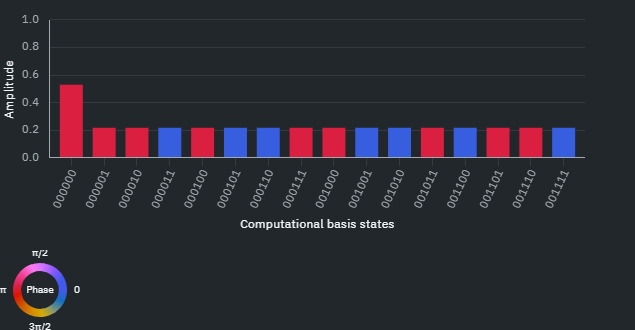
\includegraphics[trim=0mm 47mm 15mm 0mm, clip, width=.6\linewidth]{Imagens/EvPsi/Psi9.png}
        \caption{Aplicação das portas \textit{Hadamard} na operação de difusão da segunda iteração.}
        \label{fig:psi9}
    
    {\small Fonte: IBM-\textit{Quantum Learning / Composer}.}
    \end{figure}

    \item Aplicar portas $X$ (Figura~\ref{fig:psi10}):
    \begin{flalign*}
        X^{\otimes 4} \ket{\psi_9} &= \ket{\psi_{10}} = \frac{7}{32} \Bigl(-\frac{17}{7} \ket{1111} - \ket{1110} - \ket{1101} + \ket{1100} - \ket{1011} + \ket{1010} + \ket{1001} && \\ & - \ket{1000} - \ket{0111} + \ket{0110} + \ket{0101} - \ket{0100} + \ket{0011} - \ket{0010} - \ket{0001} + \ket{0000} \Bigr) && \\[6pt] 
        &= \frac{7}{32} \Bigl( \ket{0000} - \ket{0001} - \ket{0010} + \ket{0011} - \ket{0100} + \ket{0101} + \ket{0110} - \ket{0111} && \\ & - \ket{1000} + \ket{1001} + \ket{1010} - \ket{1011} + \ket{1100} - \ket{1101} - \ket{1110} - \frac{17}{7} \ket{1111} \Bigr)
    \end{flalign*}
    \vspace{-30pt}
    \begin{figure}[ht!]
        \centering
        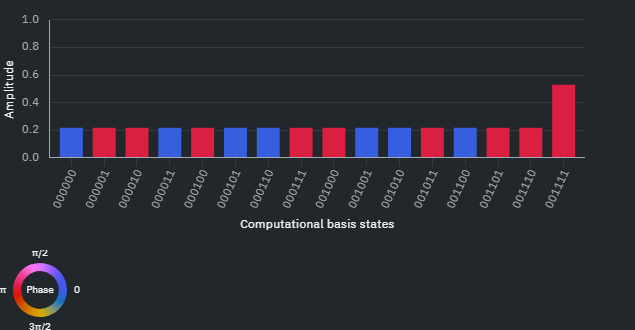
\includegraphics[trim=0mm 47mm 15mm 0mm, clip, width=.6\linewidth]{Imagens/EvPsi/Psi10.png}
        \caption{Aplicação das portas $X$ no operador de difusão da segunda iteração.}
        \label{fig:psi10}
    
    {\small Fonte: IBM-\textit{Quantum Learning / Composer}.}
    \end{figure}

    \item Aplicar porta $MCZ$ (Figura~\ref{fig:psi11}):
    \begin{flalign*}
        MCZ \ket{\psi_{10}} &= \ket{\psi_{11}} = \frac{7}{32} \Bigl( \ket{0000} - \ket{0001} - \ket{0010} + \ket{0011} - \ket{0100} + \ket{0101} + \ket{0110} && \\ 
        - \ket{0111} & - \ket{1000} + \ket{1001} + \ket{1010} - \ket{1011} + \ket{1100} - \ket{1101} - \ket{1110} + \frac{17}{7} \ket{1111} \Bigr)
    \end{flalign*}
    \vspace{-30pt}
    \begin{figure}[ht!]
        \centering
        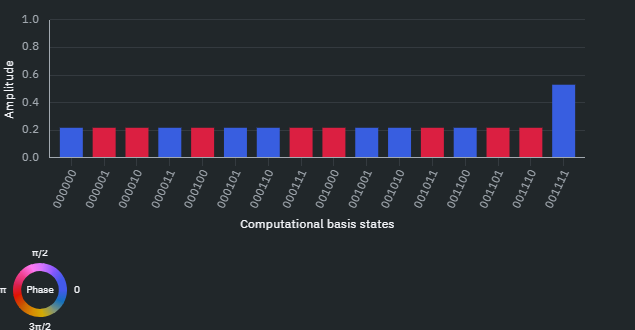
\includegraphics[trim=0mm 47mm 15mm 0mm, clip, width=.6\linewidth]{Imagens/EvPsi/Psi11.png}
        \caption{Aplicação da porta $MCZ$ na segunda iteração do operador de difusão.}
        \label{fig:psi11}
    
    {\small Fonte: IBM-\textit{Quantum Learning / Composer}.}
    \end{figure}

    \item Aplicar portas $X$ novamente (Figura~\ref{fig:psi12}):
    \begin{flalign*}
        X^{\otimes 4} \ket{\psi_{11}} &= \ket{\psi_{12}} = \frac{7}{32} \Bigl( \ket{1111} - \ket{1110} - \ket{1101} + \ket{1100} - \ket{1011} + \ket{1010} + \ket{1001} && \\ - \ket{1000} & - \ket{0111} + \ket{0110} + \ket{0101} - \ket{0100} + \ket{0011} - \ket{0010} - \ket{0001} + \frac{17}{7} \ket{0000} \Bigr) && \\[6pt]
        &= \frac{7}{32} \Bigl( \frac{17}{7} \ket{0000} - \ket{0001} - \ket{0010} + \ket{0011} - \ket{0100} + \ket{0101} + \ket{0110} - \ket{0111}  && \\ & - \ket{1000} + \ket{1001} + \ket{1010} - \ket{1011} + \ket{1100} - \ket{1101} - \ket{1110} + \ket{1111} \Bigr)
    \end{flalign*}
    \vspace{-30pt}
    \begin{figure}[ht!]
        \centering
        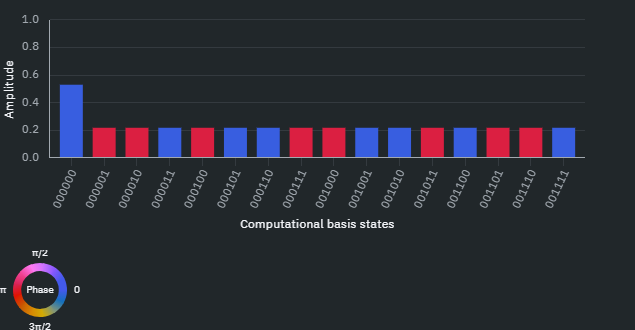
\includegraphics[trim=0mm 47mm 15mm 0mm, clip, width=.6\linewidth]{Imagens/EvPsi/Psi12.png}
        \caption{Segunda aplicação das portas $X$ na segunda iteração do operador de difusão.}
        \label{fig:psi12}
   
    {\small Fonte: IBM-\textit{Quantum Learning / Composer}.}
    \end{figure}

\item Para finalizar a segunda iteração, aplicamos novamente as portas \textit{Hadamard}:
    \begin{flalign*}
        H^{\otimes 4}\ket{\psi_{12}} &= \ket{\psi_{13}} = \frac{5}{64} \Bigl(\ket{0000}+ \ket{0001}+ \ket{0010} + \ket{0011} + \ket{0100} + \ket{0101} + \ket{0110} && \\ + \ket{0111} & + \ket{1000} + \ket{1001} + \ket{1010} + \ket{1011} + \ket{1100} + \ket{1101} + \ket{1110} + \frac{61}{5}\ket{1111}\Bigr)
    \end{flalign*}
    \vspace{-30pt}
    \begin{figure}[ht!]
        \centering
        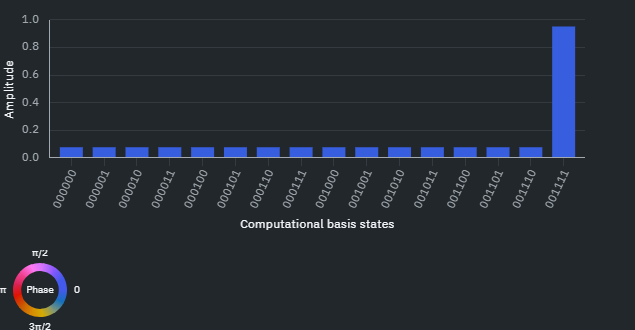
\includegraphics[trim=0mm 47mm 15mm 0mm, clip, width=.6\linewidth]{Imagens/EvPsi/Psi13.png}
        \caption{Aplicação final das portas \textit{Hadamard} na segunda iteração.}
        \label{fig:psi13}
    
    {\small Fonte: IBM-\textit{Quantum Learning / Composer}.}
    \end{figure}

O décimo terceiro passo finaliza a segunda iteração, mas é necessário repetir o processo mais uma vez.

    \item Aplicar o oráculo \(U_f\) mais uma vez (Figura~\ref{fig:psi14}):
    \begin{flalign*}
        U_f\ket{\psi_{13}} &= \ket{\psi_{14}} = \frac{5}{64} (\ket{0000} + \ket{0001} + \ket{0010} + \ket{0011} + \ket{0100} + \ket{0101} + \ket{0110} && \\ + \ket{0111}
        &+ \ket{1000} + \ket{1001} + \ket{1010} + \ket{1011} + \ket{1100} + \ket{1101} + \ket{1110} - \frac{61}{5}\ket{1111}))   
        \end{flalign*}
    \vspace{-30pt}
    \begin{figure}[ht!]
        \centering
        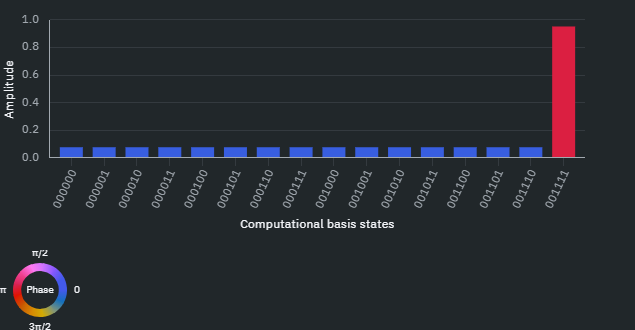
\includegraphics[trim=0mm 47mm 15mm 0mm, clip, width=.6\linewidth]{Imagens/EvPsi/Psi14.png}
        \caption{Aplicação do oráculo \(U_f\) na terceira iteração.}
        \label{fig:psi14}
    
    {\small Fonte: IBM-\textit{Quantum Learning / Composer}.}
    \end{figure}

    \item Aplicar portas \textit{Hadamard} (Figura~\ref{fig:psi15}):
    \begin{flalign*}
  H^{\otimes 4}\ket{\psi_{14}} &= \ket{\psi_{15}} = \frac{33}{128} \Bigl(\frac{7}{33}\ket{0000} + \ket{0001} + \ket{0010} -\ket{0011} + \ket{0100} - \ket{0101} -\ket{0110} && \\ 
  + \ket{0111} & + \ket{1000} -\ket{1001} -\ket{1010} + \ket{1011} - \ket{1100} + \ket{1101} + \ket{1110} - \ket{1111}\Bigr)
        \end{flalign*}
    \vspace{-30pt}
    \begin{figure}[ht!]
        \centering
        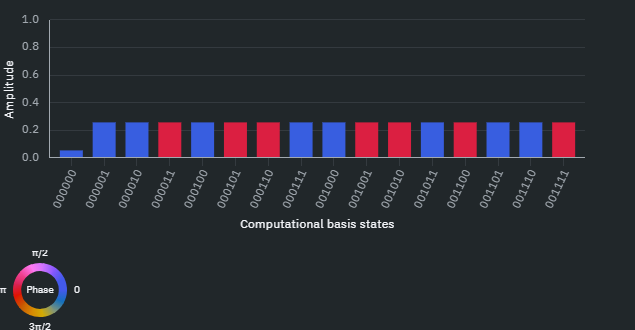
\includegraphics[trim=0mm 47mm 15mm 0mm, clip, width=.6\linewidth]{Imagens/EvPsi/Psi15.png}
        \caption{Aplicação das portas \textit{Hadamard} na operação de difusão da terceira iteração.}
        \label{fig:psi15}
    
    {\small Fonte: IBM-\textit{Quantum Learning / Composer}.}
    \end{figure}

    \item Aplicar portas $X$ (Figura~\ref{fig:psi16}):
    \begin{flalign*}
        X^{\otimes 3}\ket{\psi_{15}} &= \ket{\psi_{16}} = \frac{33}{128} \Bigl(\frac{7}{33}\ket{1111} + \ket{1110} + \ket{1101} - \ket{1100} + \ket{1011} - \ket{1010} -\ket{1001} && \\ & 
        + \ket{1000} + \ket{0111} -\ket{0110} -\ket{0101} - \ket{0100} - \ket{0011} + \ket{0010} + \ket{0001} - \ket{0000}) 
        && \\
        &= \frac{33}{128} (-\ket{0000} + \ket{0001} + \ket{0010} -\ket{0011} + \ket{0100} - \ket{0101} - \ket{0110} + \ket{0111} 
        && \\ &
        + \ket{1000} -\ket{1001} -\ket{1010} + \ket{1011} - \ket{1100} + \ket{1101} + \ket{1110} + \frac{7}{33}\ket{1111})
    \end{flalign*}
    \vspace{-30pt}
    \begin{figure}[ht!]
        \centering
        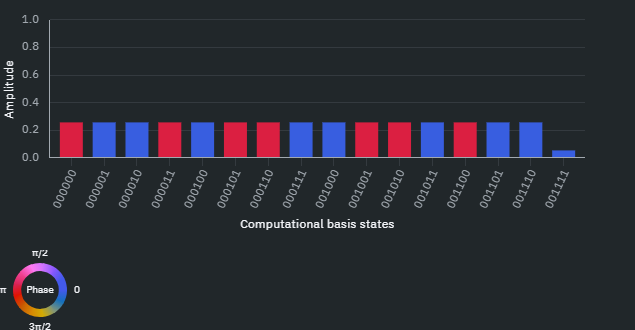
\includegraphics[trim=0mm 47mm 15mm 0mm, clip, width=.6\linewidth]{Imagens/EvPsi/Psi16.png}
        \caption{Aplicação das portas $X$ no operador de difusão da terceira iteração.}
        \label{fig:psi16}
    
    {\small Fonte: IBM-\textit{Quantum Learning / Composer}.}
    \end{figure}

    \item Aplicar porta $MCZ$ (Figura~\ref{fig:psi17}):
    \begin{flalign*}
     MCZ\ket{\psi_{16}} = \ket{\psi_{17}} = \frac{33}{128} \Bigl(&-\ket{0000} + \ket{0001} + \ket{0010} - \ket{0011} + \ket{0100} - \ket{0101} 
     && \\ &
     - \ket{0110} + \ket{0111} + \ket{1000} - \ket{1001} - \ket{1010} 
     && \\ &
     + \ket{1011} - \ket{1100} + \ket{1101} + \ket{1110} - \frac{7}{33}\ket{1111}\Bigr)    
        \end{flalign*}
    \vspace{-30pt}
    \begin{figure}[ht!]
        \centering
        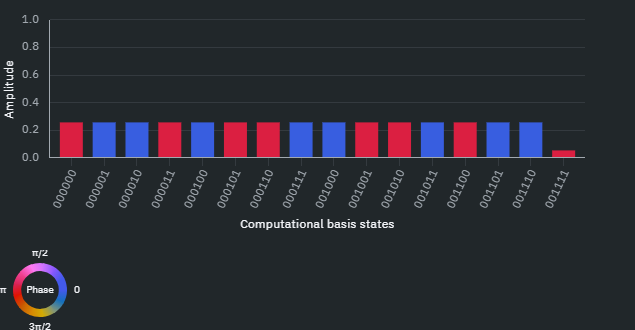
\includegraphics[trim=0mm 47mm 15mm 0mm, clip , width=.6\linewidth]{Imagens/EvPsi/Psi17.png}
        \caption{Aplicação da porta $MCZ$ na terceira iteração do operador de difusão.}
        \label{fig:psi17}
    
    {\small Fonte: IBM-\textit{Quantum Learning / Composer}.}
    \end{figure}

    \item Aplicar portas $X$ (Figura~\ref{fig:psi18}):
    \begin{flalign*}
         X^{4}\ket{\psi_{17}} = \ket{\psi_{18}} = \frac{33}{128} \Bigl(&-\ket{1111}  + \ket{1110}  + \ket{1101} - \ket{1100}  + \ket{1011} 
         && \\ &
         - \ket{1010} - \ket{1001}  + \ket{1000}  + \ket{0111} - \ket{0110} - \ket{0101}  && \\ & + \ket{0100} - \ket{0011}  + \ket{0010}  + \ket{0001} - \frac{7}{33}\ket{0000}\Bigr) 
         && \\
         = \frac{33}{128} \Bigl(&-\frac{7}{33}\ket{0000}  + \ket{0001}  + \ket{0010} - \ket{0011}  && \\ & 
         + \ket{0100} - \ket{0101} - \ket{0110}  + \ket{0111}  + \ket{1000} - \ket{1001} && \\ &
         - \ket{1010}  + \ket{1011} - \ket{1100}  + \ket{1101}  + \ket{1110} - \ket{1111}\Bigr)
    \end{flalign*}
    \vspace{-30pt}
    \begin{figure}[ht!]
        \centering
        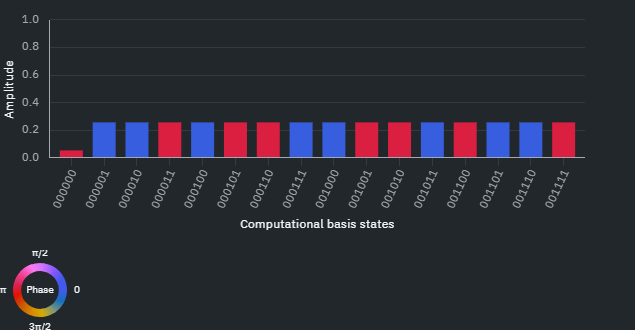
\includegraphics[trim=0mm 47mm 15mm 0mm, clip, width=.6\linewidth]{Imagens/EvPsi/Psi18.png}
        \caption{Última aplicação das portas $X$ na terceira iteração do operador de difusão.}
        \label{fig:psi18}

    {\small Fonte: IBM-\textit{Quantum Learning / Composer}.}
    \end{figure}

        \item Para finalizar a terceira e última iteração, aplicamos novamente as portas \textit{Hadamard} (Figura~\ref{fig:psi19}):
    \begin{flalign*}
         H^{\otimes 4}\ket{\psi_{19}} = \ket{\psi_{20}} = \frac{13}{256} \Bigl(&\ket{0000} + \ket{0001} + \ket{0010} + \ket{0011} + \ket{0100} + \ket{0101} && \\ & 
         + \ket{0110} + \ket{0111} + \ket{1000} + \ket{1001} + \ket{1010} + \ket{1011} && \\ &
         + \ket{1100} + \ket{1101} + \ket{1110} - \frac{251}{13}\ket{1111}\Bigr) 
        \end{flalign*}
    \vspace{-30pt}
    \begin{figure}[ht!]
        \centering
        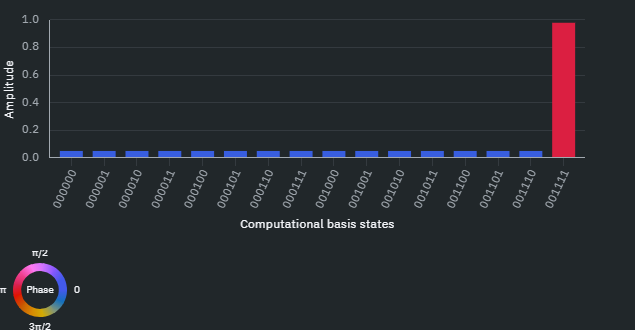
\includegraphics[trim=0mm 47mm 15mm 0mm, clip, width=.6\linewidth]{Imagens/EvPsi/Psi19.png}
        \caption{Probabilidades finais de \(\ket{\psi}\) após as três iterações do Algoritmo de Grover.}
        \label{fig:psi19}

    {\small Fonte: IBM-\textit{Quantum Learning / Composer}.}
    \end{figure}

\end{enumerate}

Ao final do processo, o estado marcado \(\ket{1111}\) aparece com amplitude máxima, o que confirma a eficiência do Algoritmo de Grover em aumentar a probabilidade do estado desejado em um espaço de busca não estruturado.

\vspace{-5pt}
\begin{figure}[ht!]
    \centering
    \captionsetup{justification=centering}    
    \caption{Amplitude e probabilidades após medição final do circuito.}
    \label{fig:AmpProbFinalComposer}
    
    \begin{subfigure}{.48\textwidth}
        \centering
        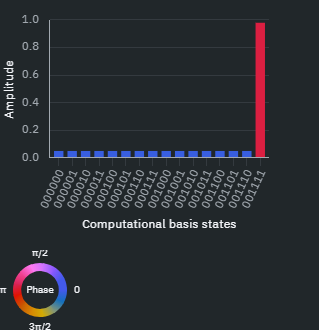
\includegraphics[trim=0mm 47mm 15mm 0mm,clip,width=.7\textwidth]{Imagens/EvPsi/amplitudeFinal.png}
        \subcaption{Amplitude do estado \(\ket{1111}\) igual a $0,98$.}
        \label{subfig:AmpFinalComposer}
    \end{subfigure}
    \begin{subfigure}{.48\textwidth}
        \centering
        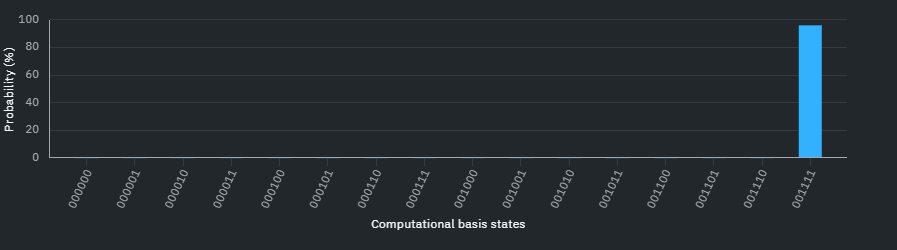
\includegraphics[trim=0mm 0mm 17mm 0mm,clip,width=\textwidth]{Imagens/EvPsi/ProbFinal.png}
        \subcaption{Probabilidades finais de cada estado do espaço de busca, com \(96{,}13\%\) para o estado \(\ket{1111}\).}
        \label{subfig:ProbFinalComposer}
    \end{subfigure}
    
    {\small Fonte: IBM-\textit{Quantum Learning / Composer}.}
\end{figure}
